\documentclass[a4paper,12pt]{report}
\usepackage[toc,page]{appendix}
\usepackage{amsmath}
\usepackage{float}
\usepackage{graphicx}
\usepackage{subfig}
\usepackage{amssymb}
\usepackage{geometry}
\usepackage{array}
\usepackage{tcolorbox}
\usepackage[normalem]{ulem}

\usepackage{setspace}
 \geometry{
 a4paper,
 total={170mm,257mm},
 left=20mm,
 top=20mm,
 }
\usepackage{tikz}
\usepackage{pgfplots}
\usetikzlibrary{shapes, arrows.meta, decorations.pathreplacing, positioning, petri, fit, calc}
\tikzstyle{startstop} = [circle, minimum size=1cm ,text centered, draw=black]
\tikzstyle{neuron} = [circle, minimum size=1cm ,text centered, draw=red, fill=gray!30]
\tikzstyle{neuronEll} = [ellipse, minimum size=1cm ,text centered, text width=2cm, draw=red, fill=gray!30]
\tikzstyle{process} = [rectangle, minimum width=2cm, minimum height=2cm, text centered, text width=5cm, draw=black, fill=blue!30]
\tikzstyle{detail} = [rectangle, minimum width=1.5cm, minimum height=0.5cm, text justified, text width=2.6cm, fill=white!30]
\tikzstyle{smalldetail} = [rectangle, minimum width=2cm, minimum height=1cm, text centered, text width=2cm]
\tikzstyle{largedetail} = [rectangle, minimum width=3cm, minimum height=1cm, text centered, text width=4cm, fill=white!30]
\tikzstyle{box} = [rectangle, minimum width=5cm, minimum height=9cm, text centered, text width=4cm, draw=black, fill=white!30]

\usepackage[utf8]{inputenc}

% Default fixed font does not support bold face
\DeclareFixedFont{\ttb}{T1}{txtt}{bx}{n}{10} % for bold
\DeclareFixedFont{\ttm}{T1}{txtt}{m}{n}{10}  % for normal

% Custom colors
\usepackage{color}
\definecolor{deepblue}{rgb}{0,0,0.5}
\definecolor{deepred}{rgb}{0.6,0,0}
\definecolor{deepgreen}{rgb}{0,0.5,0}

\usepackage{listings}
\usepackage{mathtools}
% Python style for highlighting
\newcommand\pythonstyle{\lstset{
language=Python,
basicstyle=\ttm,
otherkeywords={self},             % Add keywords here
keywordstyle=\ttb\color{deepblue},
emph={MyClass,__init__},          % Custom highlighting
emphstyle=\ttb\color{deepred},    % Custom highlighting style
stringstyle=\color{deepgreen},
frame=tb,                         % Any extra options here
showstringspaces=false            % 
}}


% Python environment
\lstnewenvironment{python}[1][]
{
\pythonstyle
\lstset{#1}
}
{}

% Python for external files
\newcommand\pythonexternal[2][]{{
\pythonstyle
\lstinputlisting[#1]{#2}}}

% Python for inline
\newcommand\pythoninline[1]{{\pythonstyle\lstinline!#1!}}


\begin{document}
\tableofcontents

\title{Application example: Photo OCR \\
Optical Character Recognition}
\maketitle
\part{Week 11}
\section{OCR Problem Description}
Photo OCR pipeline:
\begin{figure}[H]
\resizebox {5in} {!} {
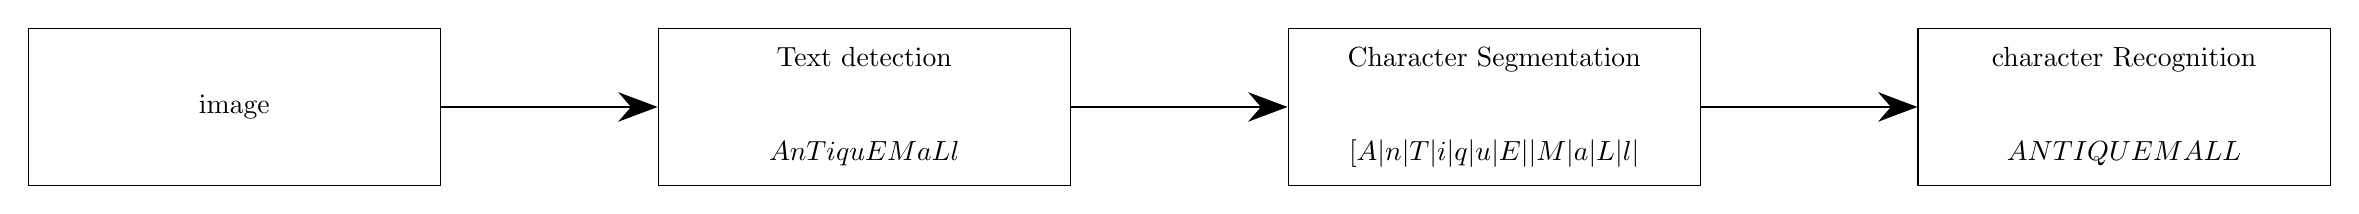
\begin{tikzpicture}[node distance=0cm]
\node (h1) [process, draw=black, fill=white!30] {image};
\node (h2) [process, below of=h1, xshift=8cm, yshift=0cm,draw=black, fill=white!30] {Text detection \\ \[AnTiquE MaLl\]};
\node (h3)[process, below of=h2, xshift=8cm, yshift=0cm,draw=black, fill=white!30] {Character Segmentation \\ \[[A|n|T|i|q|u|E| |M|a|L|l|\] };
\node (h4)[process, below of=h3, xshift=8cm, yshift=0cm,draw=black, fill=white!30] {character Recognition \\ \[ANTIQUE MALL\] };
\draw[-{Stealth[length=5mm]}](h1) -- (h2);
\draw[-{Stealth[length=5mm]}] (h2) -- (h3);
\draw[-{Stealth[length=5mm]}] (h3) -- (h4);
\end{tikzpicture}
}
\end{figure}
\begin{enumerate}
\item text detection using sliding window:
\begin{itemize}
\item use a labeled training set with positive examples ($y=1$) when image is a text and $y=0$ (negative example), the image has not text.
\item the resulting image is a black and white image where the positive example are white
\item Once  text objects are detected, apply "expansion operation": this expands the white region for every pixel if the neighbouring white pixel is close
\end{itemize}
\item Character segmentation:
\begin{itemize}
\item Use supervised learning algorithm to look for gap in between letters : positive example $y=1$ is an image with a gap between 2 letters.
\end{itemize}
\item Character recognition is performed using 1D sliding window
\end{enumerate}
\subsection{Sliding window for Pedestrian Detection}
\begin{itemize}
	\item This is a supervised learning, where the NN is trained on labeled images : image of pedestrian $y=1$, image without pedestrian $y=0$).
	\item on a test set image, we take a patch (green box below) and determine if $y=1$ or $y=0$, and move the box by pre-determined step-size: this is called \textbf{sliding window}
	\item we then increase the patch size
\end{itemize}
\begin{figure}[H]
\includegraphics[scale=0.5]{pedestrian.pdf}
\end{figure}

\section{Artificial Data Synthesis}
There are 2 techniques to new new data:
\begin{itemize}
\item create new data from scratch
\item synthesizing data by introducing artificial distorsions
\end{itemize}
This works for image, but also speech recognition (by introducing noise, background). Note that the distorsion introduced should be representation of the type of noise/distorsions in the test data. However, usually it does not help to add purely random/meaningless noise to the data ($x \leftarrow x + \text{random \ noise}$

\section{Ceiling Analysis}
With Ceiling Analysis, we estimate the errors due to each component of the pipeline, which helps determining what component is more likely to improve the overall model. \\

We illustrate the concept using OCR pipeline
\begin{figure}[H]
\resizebox {5in} {!} {
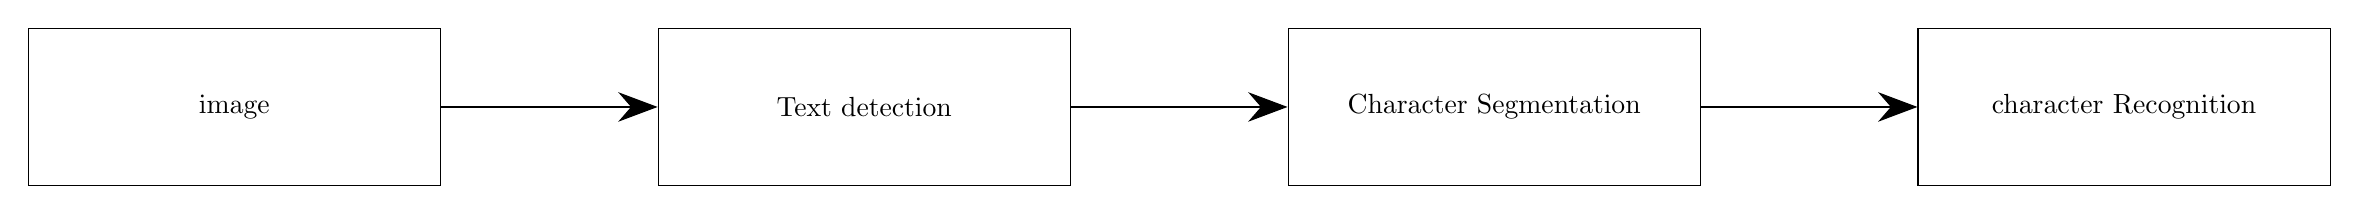
\begin{tikzpicture}[node distance=0cm]
\node (h1) [process, draw=black, fill=white!30] {image};
\node (h2) [process, below of=h1, xshift=8cm, yshift=0cm,draw=black, fill=white!30] {Text detection };
\node (h3)[process, below of=h2, xshift=8cm, yshift=0cm,draw=black, fill=white!30] {Character Segmentation  };
\node (h4)[process, below of=h3, xshift=8cm, yshift=0cm,draw=black, fill=white!30] {character Recognition };
\draw[-{Stealth[length=5mm]}](h1) -- (h2);
\draw[-{Stealth[length=5mm]}] (h2) -- (h3);
\draw[-{Stealth[length=5mm]}] (h3) -- (h4);
\end{tikzpicture}
}
\end{figure}

\begin{table}[H]
\begin{tabular}{||c|c||}
\hline
\textbf{component} & \textbf{accuracy test set} \\
\hline
overall system & 72\% \\
\hline
Text detection & 89\% \\
plugging in the ground truth labels of the test set & \\
i.e making text detection 100\% accurate & \\
\hline
(Manually) Character Segmentatiton & 90\% \\
\hline
(Manually) character recognition & 100\% \\
\hline
\end{tabular}
\end{table}
The largest improvement is obtained with improving "Text Detection". 
\end{document}